\chapter{Chat with PPP data}
%cite{w15} is a problem why?

\section{Introduction}
%This chapter delves into the innovative integration of LLMs (Large Language Models) technology with PPP (Public-Private Partnership) project data. The fusion of AI-driven chat capabilities with PPP data is designed to enhance the feasibility analysis process, providing stakeholders with a more dynamic, interactive, and informed decision-making tool. By leveraging the Retrieval Augmented Generation (RAG) model, this approach aims to significantly improve the precision and relevance of generated responses, tailored to the specific needs and complexities of PPP projects.
This chapter explores the innovative application of Large Language Models (LLMs) combined with Public-Private Partnership (PPP) data in project management. To improve the feasibility analysis process, AI-driven chat capabilities are integrated with PPP data, offering stakeholders a dynamic, interactive, and informed decision-making tool. Additionally, a Retrieval Augmented Generation (RAG) model is employed to enhance the precision and relevance of the responses generated, specifically tailored to meet the unique needs and complexities of PPP projects.
\section{Problem}
%Public-Private Partnership (PPP) projects generate vast amounts of data, from detailed financial reports to comprehensive performance reports. Analyzing this wealth of historical data for insights is a formidable challenge, crucial for refining future PPP ventures. Traditional data analysis methods are often inadequate due to the sheer volume of data, leading to potential oversights and a failure to harness valuable lessons learned.
PPP projects create a lot of information, like financial and performance reports. Studying all this old information to find helpful ideas is a big task, important for improving upcoming partnerships. Traditional data analysis methods may not be enough because of too much data, which can cause important information to be missed or not used effectively. 
\vskip 0.5cm
%Moreover, the relevance of data from past projects diminishes without the ability to adapt insights to the evolving landscapes of regulations, market conditions, and technological advances. As a result, critical decision-making, risk management, and project planning suffer, impacting the efficiency and success of future PPP initiatives.
Furthermore, data from old projects becomes less useful without being able to apply lessons to new rules, market changes, and technology progress. As a result, important choices, making sure things go smoothly, and planning future projects are affected, which makes it harder for future PPP initiatives to be successful.
\vskip 0.5cm
%Addressing this problem requires a novel solution capable of digesting extensive historical data and extracting pertinent insights efficiently. Chatbots, especially those powered by advanced AI algorithms, emerge as a promising solution. They can automate the analysis of large datasets, offer real-time insights, and adapt learnings to the specific context of new PPP projects. By leveraging chatbots, stakeholders can unlock the full potential of their historical data, guiding more informed and effective future project planning and execution. But we must decide what is the best type of chat-bot to use based on our dataset.
To solve this problem, we need a new idea that can analyze a lot of old information and find important information quickly. Chatbots, especially those powered by advanced AI algorithms, are becoming a very good solution. They can automate the analysis of big sets of data, provide immediate insights, and adjust learnings to the specific situation of new PPP projects. By using chatbots, people can make the most of their old data and make better plans for future projects. But we must choose the best type of chat bot to use based on our information.
\section{The Dataset}
Our dataset,a sample was shown at \textbf{Figure \ref{fig:dataset}}, taken from PPP projects, is mostly semi-structured, with Word documents that have text, tables, and images. This type has unique features and information that make it difficult to manage and analyze data efficiently.
%Our dataset, derived from Public-Private Partnership (PPP) projects, is fundamentally semi-structured, containing Word documents that integrate text, tables, and images. This variety poses distinct challenges in data management and analysis, given the unique attributes and insights each data type offers.
\vskip 0.5cm
\begin{figure}[H]
    
    \centering
    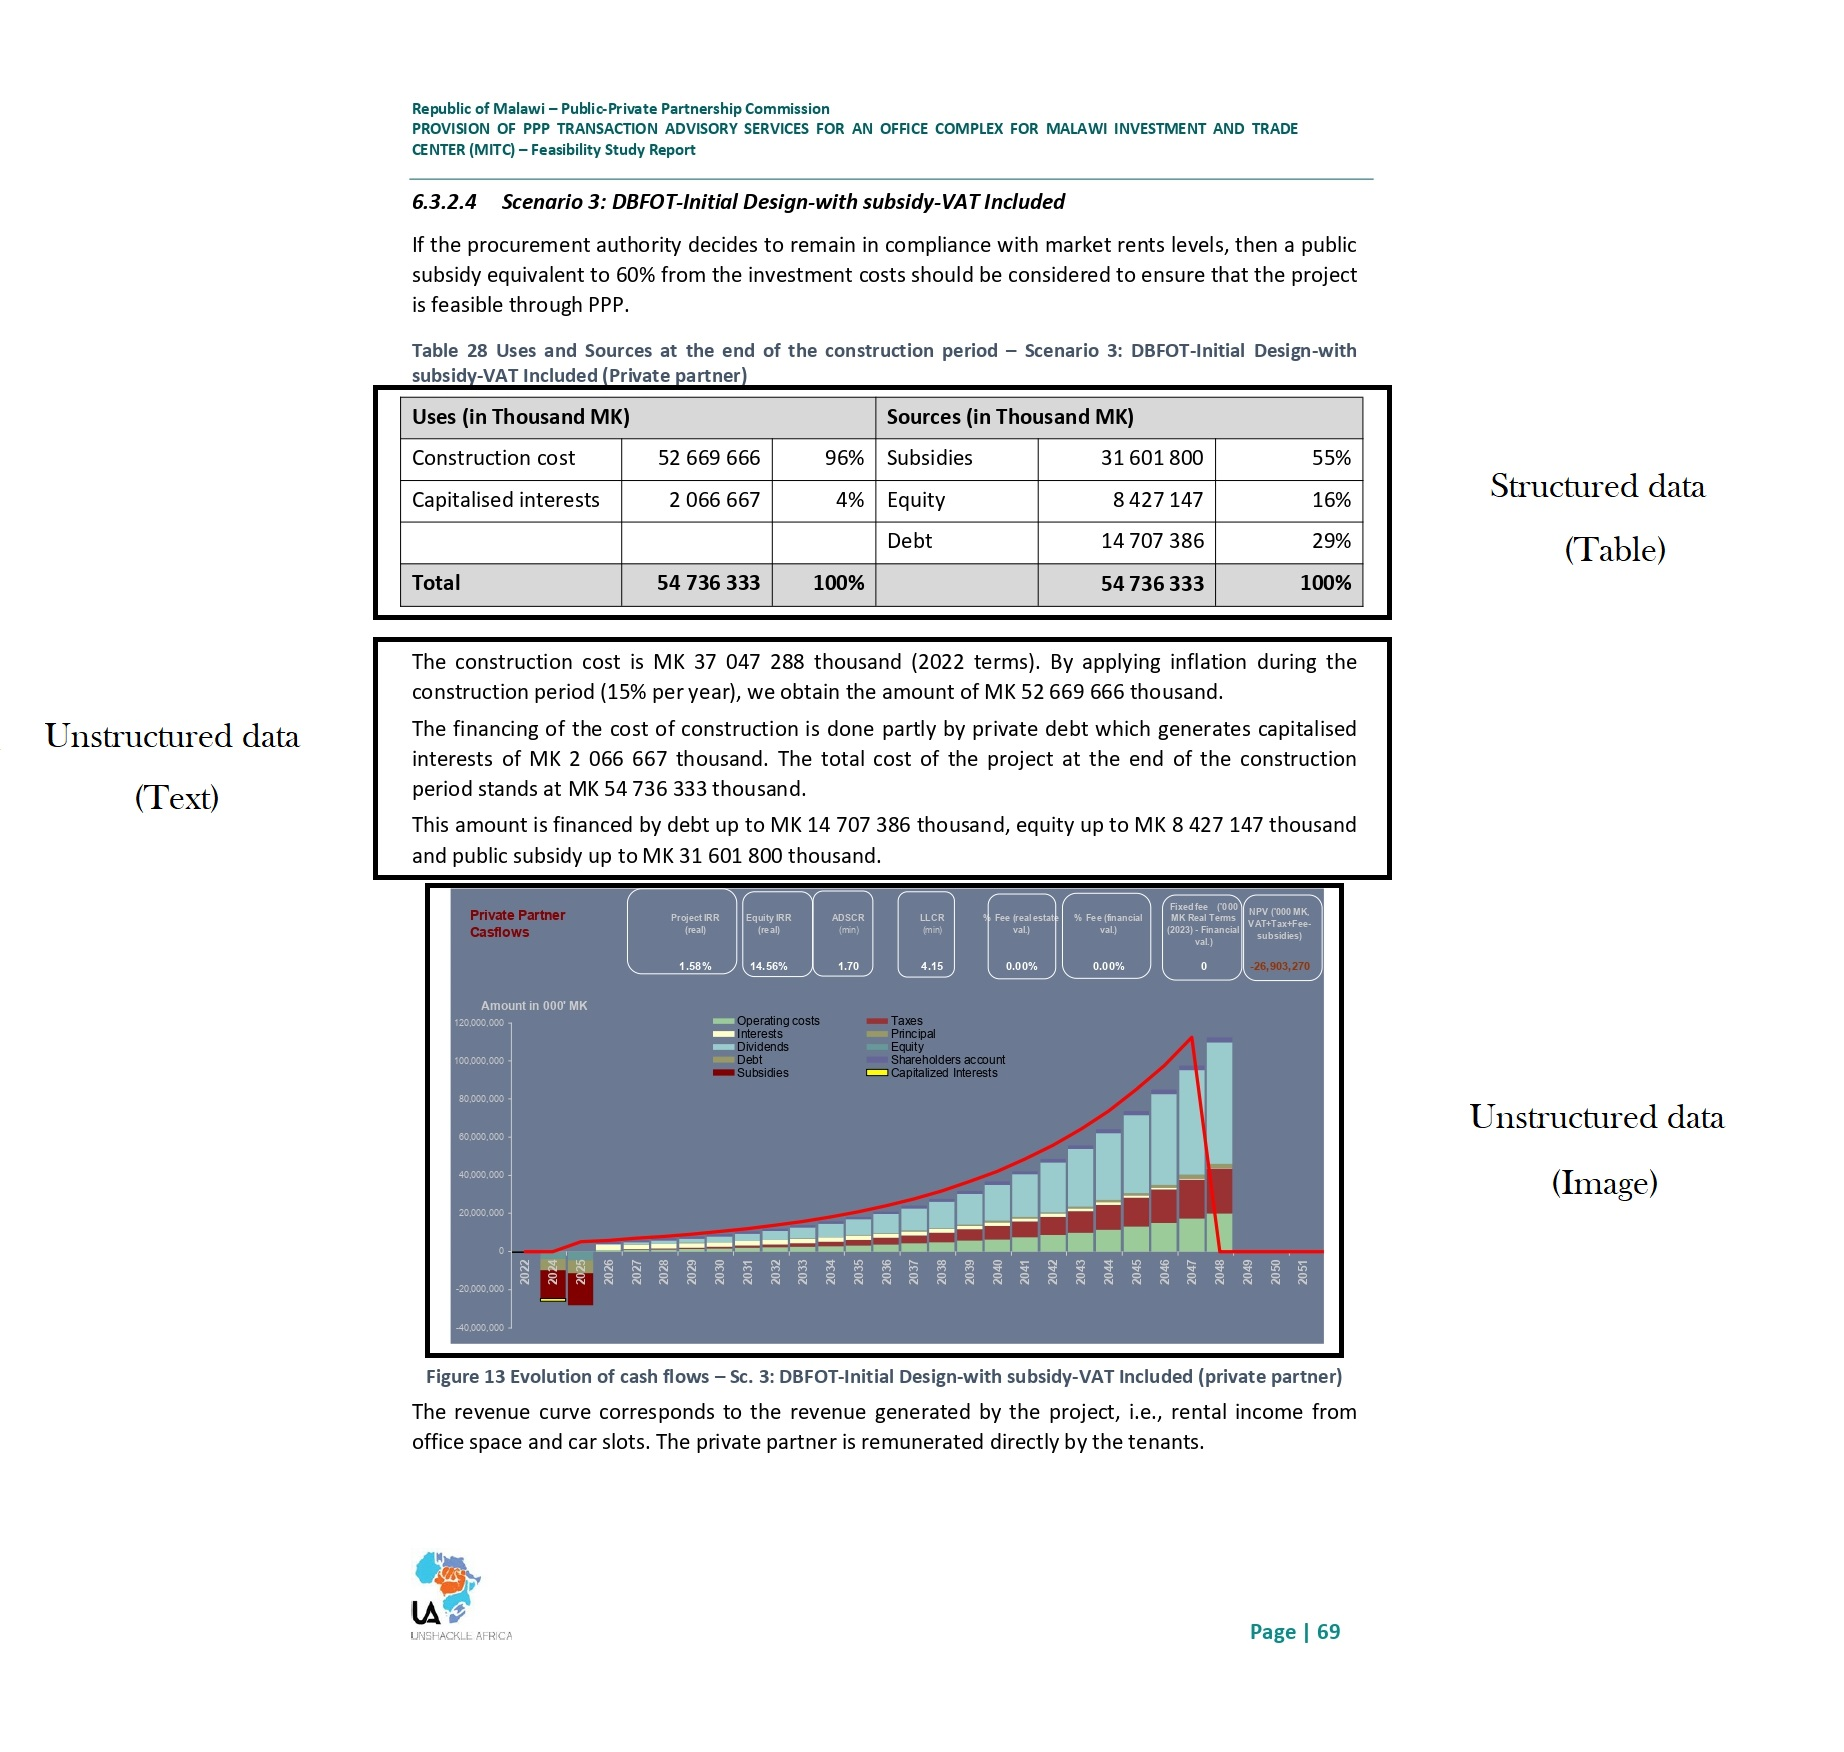
\includegraphics[width=1 \linewidth]{assets/data_ex_page-0001.jpg}
    \caption{Example of a dataset page}
    \label{fig:dataset}
\end{figure}
\vskip 0.5cm
Text: The textual data The textual data includes all the information about projects, contracts, reports on progress, and messages to people involved in the project. The text is full of details but it's hard for computers to understand because it doesn't have a clear structure. Understanding and interpreting detailed documents to find useful information can be difficult because of the complex language and jargon used in PPP projects.
%Text: The textual data includes detailed project descriptions, contracts, progress reports, and stakeholder communications. While rich in narrative detail, the text presents a challenge for automated processing due to its unstructured nature. Extracting specific insights or actionable information from lengthy documents requires sophisticated understanding and interpretation, often complicated by the technical language and specific jargon used in PPP projects.
\vskip 0.5cm
Tables: Embedded within documents, tables give important, organized information about finances, schedules, and performance indicators. The issue comes from the different ways the tables are set up and used in the text. Automated tools need to figure out and take out important information without losing the meaning given by the surrounding text, which can be difficult because of the different layouts and designs used in documents.
%Tables: Embedded within the documents, tables provide crucial, structured data on financials, schedules, and performance indicators. The problem arises in the inconsistent formatting and contextual embedding of these tables. Automated tools must discern and extract relevant data without losing the context provided by accompanying text, a task complicated by the varied layouts and designs employed across documents.
\vskip 0.5cm
Pictures: Pictures, like project drawings, graphs, and photos of the site, give important information about how the project is going and what the results are. Their study is limited because they require special processing methods. Taking information from pictures, especially when it has words or complicated visuals, needs high-tech OCR and image recognition tools, which may have trouble with picture quality, direction, and combining visual data with text and tables.
%Images: Images, including project visualizations, charts, and site photographs, offer valuable insights into project progress and outcomes. However, their analysis is hindered by the need for specialized processing techniques. Extracting data from images, particularly when it involves text or complex visual information, requires advanced OCR and image recognition technologies, which can struggle with image quality, orientation, and the integration of visual data with textual and tabular information.
\vskip 0.5cm
The variety and semi-structered data of our dataset show how complicated it is to analyze data from PPP projects. The difficulties include:
%The diversity and semi-structured nature of our dataset underscore the complexities inherent in PPP project data analysis. The challenges include:
\vskip 0.5cm
Data Integration: Combining information from text, tables, and pictures to better understand project progress and results.%Combining insights from text, tables, and images into a coherent understanding of project statuses and outcomes.
Context Preservation: Keeping the connections between different types of information, like the story behind a table or the details about an image, is very important for getting the analysis right.%Maintaining the context between data types, such as the narrative explanation of a table or the description tied to an image, is crucial for accurate analysis.
Format Variability: There are many different types of documents that need flexible tools to deal with them.
Technical Language: The terminology and common terms in PPP papers need really smart AI tools to understand them correctly.
\vskip 0.5cm
%Addressing these challenges requires a nuanced approach to data processing and analysis, emphasizing the need for advanced tools like chat bots capable of navigating the complexities of semi-structured PPP project data.
Dealing with these challenges requires advanced tools like chat bots that can handle complex PPP project data in a nuanced way. This helps in processing and analyzing data effectively.

\section{Types of Chat-bots}
In the context of managing and analyzing PPP data, it is important to know the different types of chatbots that you can use. These can be put into two groups: rule based chatbots and AI driven chatbots. Each one has its own specific uses and levels of difficulty and flexibility.
%In the context of managing and analyzing Public-Private Partnership (PPP) data, understanding the different types of chatbots available is crucial. These can be broadly categorized into rule-based chatbots and AI-driven chatbots, each serving unique purposes and offering varying levels of complexity and adaptability:
\vskip 0.5cm
\begin{itemize}
\item \textbf{Rule-Based Chatbots:} These chatbots work based on a specific set of rules. They are designed for simple and predictable conversations. Rule-based chatbots excel in scenarios where queries fall within a well-defined range, making them efficient for FAQ-style interactions. However, using to analyze PPP data is difficult because the data is complex and can vary a lot. They are not able to handle unstructured data or give insights beyond their set rules.
%Rule-Based Chatbots: These chatbots operate on a set of predefined rules. They are designed to handle straightforward, structured conversations where responses can be predicted. Rule-based chatbots excel in scenarios where queries fall within a well-defined range, making them efficient for FAQ-style interactions. However, their application in analyzing PPP data is limited due to the complexity and variability of the data involved. They lack the flexibility to process unstructured data or provide insights beyond their programmed rules.
\vskip 0.5cm
\item \textbf{NLP-Driven Chatbots:} AI-driven chatbots, powered by machine learning and natural language processing NLP , can understand and interpret the nuances of human language. Unlike their rule based counterparts, they learn from interactions to improve their understanding over time, making them capable of handling unstructured data. In the world of PPP projects, AI-powered chatbots can look at a lot of insights, find patterns, and get useful information from previous project documents. Their skill in handling and understanding lots of difficult data makes them great at giving personalized advice and predicting future outcomes for projects.
%AI-Driven Chatbots: Powered by machine learning and natural language processing (NLP), AI-driven chatbots can understand and interpret the nuances of human language. Unlike their rule-based counterparts, they learn from interactions to improve their understanding over time, making them capable of handling unstructured data. In the realm of PPP projects, AI-driven chatbots can analyze extensive datasets, identify patterns, and extract actionable insights from past project documentation. Their ability to process and learn from large volumes of complex data makes them particularly suited for offering tailored advice and predictive analytics for future projects.
\vskip 0.5cm
\item \textbf{Hybrid Chatbots:} Using elements from two different methods, hybrid chatbots can answer simple questions using set rules and switch to more advanced answers using artificial intelligence for harder questions. This method ensures that we handle basic questions efficiently and consistently, while still having the ability to dig deeper into data and generate insights for PPP projects.
%Hybrid Chatbots: Combining the best of both worlds, hybrid chatbots utilize rule-based systems for handling routine inquiries and switch to AI-driven responses for more complex questions. This approach ensures efficiency and consistency in dealing with standard queries while retaining the flexibility to engage in more sophisticated data analysis and insight generation related to PPP projects.
\vskip 0.5cm

\item \textbf{Retrieval-Augmented Generation (RAG) Chatbots:} RAG chatbots are a type of AI chatbots that are really good at finding information from a big database before coming up with answers. Chatbots use information from previous projects to give helpful advice and predictions about future projects. Their ability to access historical data archives makes them extremely useful for understanding complicated PPP data environments.
%Retrieval-Augmented Generation (RAG) Chatbots: A subcategory of AI-driven chatbots, RAG chatbots specialize in retrieving information from a vast database before generating responses. By consulting specific data points from past PPP projects, these chatbots can provide highly relevant and context-aware insights, advice, and foresight on potential project outcomes. Their capability to tap directly into historical data archives makes them invaluable for deciphering complex PPP data landscapes.
\end{itemize}
\vskip 0.5cm
In the context of tackling the challenges presented by PPP data analysis, AI-driven and RAG chatbots hold the most promise. Their ability to process and learn from unstructured data, combined with the capability to retrieve and utilize specific information from large datasets, positions them as powerful tools for extracting insights from historical PPP project data. This, in turn, can significantly enhance decision-making and strategic planning for future projects.

\section{Why RAG}
Retrival Augmented Generation RAG mixes the Advanced text-generation skills of GPT and other large language models with information searching features to give correct and contextually relevant information. This new method helps language models better understand and respond to user questions by using the most up-to-date information available. As RAG grows, its many uses are going to change how well AI works and how useful it is.
%Retrieval Augmented Generation (RAG) combines the advanced text-generation capabilities of GPT and other large language models with information retrieval functions to provide precise and contextually relevant information. This innovative approach improves language models' ability to understand and process user queries by integrating the latest and most relevant data. As RAG continues to evolve, its growing applications are set to revolutionize AI efficiency and utility.
\vskip 0.5cm
%In general, General-purpose language models are pre-trained on vast amounts of data from everywhere. But this doesn't mean that it knows the answer to every question. General LLMs fall short in cases like up-to-date or relevant information, domain-specific context, fact-checking, etc. That's why they're called general-purpose and need the assistance of other techniques that are widely implemented to make LLMs more versatile.
%Therefore, we address these shortcomings by integrating information retrieval mechanisms, enabling language models to access external knowledge sources for more accurate and relevant responses, thus mitigate hallucination and strengthen reliability.
In general, General-purpose language models are trained on a lot of data from everywhere. But doesn't mean it knows the answer to every question. Traditional LLMs lack important things like current or important information, specific context, fact checking, etc. That's why they re-called general purpose and need the help of other widely used techniques to make LLMs more versatile.
So, we fix these problems by adding ways for language models to find information, so they can give better and more specific answers. This helps prevent them from making things up and makes them more trustworthy.

\section{Our RAG Components and Pipeline}
%In this section, we will examine the intricate components and sequential processes that constitute our Retrieval-Augmented Generation (RAG) pipeline. We managed to create this pipeline after many iterations of testing and evaluation so we can have the best results. This pipeline stands at the core of our chatbot's ability to navigate through and interact with the multi-faceted data associated with Public-Private Partnership (PPP) projects. It is a harmonious interplay of extraction, indexing, retrieval, fusion, and generation modules, each fine-tuned to handle the semi-structured nature of the PPP data sets, which include text and tables within Word documents, we can see the pipline in figure 4.1.
In this part, we will look at the detailed parts and steps that make up our Retrieval Augmented Generation RAG pipeline. We made this pipeline after lots of testing and evaluation to get the best results. This pipeline is crucial for our chatbot to move through and communicate with the complex data linked to Public Private Partnership PPP projects. It is a smooth combination of different parts that work together to process PPP data sets, which contain text and tables within Word documents. \textbf{Figure \ref{fig:our_rag}} shows the pipeline.
\begin{figure}[H]
    \centering
    \includegraphics[width=1 \linewidth]{assets/our_rag.png}
    \caption{Our RAG pipline}
    \label{fig:our_rag}
\end{figure}

Based on this pipline, in this chapter we will talk about:
\vskip 0.5cm
\begin{itemize}
\item \textbf{Data Extraction and Preparation:} This step involves identifying and extracting out different types of information from Word documents. This includes text and tables. The process makes sure that all important information is gathered and ready for the next steps.%This step involves identifying and extracting varied data types from the Word documents, including text and tables. The process ensures that all relevant information is captured and prepared for the subsequent steps in the pipeline.
\vskip 0.5cm
\item \textbf{Data Embedding}: After extraction, the data goes through a process called embedding. This changes the information into numbers that AI can easily understand and work with. This embedding is very important for capturing the meaning of the data in a way that machines can understand and use it effectively. %After extraction, the data undergoes embedding, where it is transformed into a numerical representation that can be efficiently processed by AI algorithms. This embedding is crucial for capturing the semantic richness of the data in a form that machines can understand and work with.
\vskip 0.5cm
\item \textbf{History-Aware Conversation Management}: At this point, the system uses past interactions to keep track of the conversation flow. This makes sure that each question is based on the history of the conversation, giving a smooth and relevant experience for the user.%At this stage, the system leverages the context of previous interactions to maintain a history-aware conversation flow. This ensures that each query builds on the last, providing continuity and relevance to the user's ongoing experience.
\vskip 0.5cm
\item \textbf{Integrated Retrieval, Indexing, and Re-Ranking}: This system begins by retrieving data from out vector store based on the users question. The retrieval process is integrated with a creative technique known as RAG Fusion. During this phase, the retrieved data is re-ranked by importance, which enhances the quality and relevance of the information used for generating answers. This integrated approach ensures efficient data handling and improved response generation for the user.
\vskip 0.5cm
\item \textbf{Answer Generation}: The last stage of the process where the chatbot puts together the re-ordered information to create complete and relevant answers. The process uses language models and data to give accurate answers to user questions.%The final step of the pipeline where the chatbot synthesizes the re-ranked data to generate comprehensive and contextually relevant responses. The generation process combines the power of language models with the specificity of retrieved data to produce accurate and informative answers to user inquiries.
\end{itemize}
\vskip 0.5cm
%This refined pipeline provides a systematic approach for transforming semi-structured PPP project data into actionable insights through a conversational AI interface. Each step is designed to handle the complexity of the data and the nuances of user interactions, ensuring that the chatbot is not only responsive but also deeply informative.
This advanced pipeline helps to change semi structured PPP project information into useful insights using a conversational AI interface. Each step is made to deal with the difficulty of the data and the details of how users interact, making sure that the chatbot is not just quick to respond but also very informative.
%https://medium.com/@sandyeep70/understanding-rag-evolution-components-implementation-and-applications-ecf72b778d15

%---------------------------------------
\section{Data Extraction and Preparation}
The text extraction stage is important in the RAG pipeline. Here, the AI system works with the Word document to find and separate all the text. This process is intricate and has many steps to make sure the text data is accurate and ready to be used.
%The text extraction stage is a critical part of the RAG pipeline where the AI system interacts with the Word document to identify and isolate the full textual content. This process is intricate and involves several steps to ensure the text data is accurate and ready for interaction.
\vskip 0.5cm
The extraction process is divided into two distinct sub-tasks, one devoted to text extraction and processing  and the other focused on tables extraction and processing This section allows essential control of each type of data, making the extraction process more accurate and efficient. By carefully analyzing textual content and tabular data, the system can gather broader perspectives and enhance its knowledge base, ultimately increasing its ability to provide contextual responses.

\subsection{Text extraction and processing}
The extraction process is divided into two parts, one for extracting and processing text, and the other for tables. This helps make sure the data is extracted accurately and quickly. By looking closely at written words and table data, the system can learn more and improve its knowledge. This helps it give better answers in different situations.
%The initial phase of the RAG pipeline's text interaction involves the comprehensive extraction and meticulous cleaning of textual content from the PPP documents, ensuring that the data fed into the system is of the highest quality and relevance.
\vskip 0.5cm
\begin{itemize}
\item \textbf{Full Text Extraction}: This process begins with a thorough scan of the entire Word document. Sophisticated algorithms are used to go through the document's complicated structure and capture all parts that have text. This means looking closely at all parts of the document, like the main text, titles, footnotes, and extra information on the side. Every paragraph, heading, and written note is carefully taken out, making sure no important information is missed.%This process starts with a deep scan of the entire Word document. Advanced parsing algorithms are deployed to navigate through the complex structure of the document, capturing every element that contains text. This includes diving into the main body, headers, footers, and side notes. Every paragraph, heading, and written note is meticulously extracted, ensuring no potential insight is left behind.
\vskip 0.5cm
This step is crucial because it sets the foundation for the kind of information the chatbot will have available. It is done carefully to capture the detailed story in PPP documents, like project goals, timelines, stakeholder duties, and legal rules.
%This step is crucial as it lays the groundwork for the kind of information the chatbot will have at its disposal. It is performed with precision to capture the nuanced narrative often present in PPP documents, which may include project goals, timelines, stakeholder responsibilities, and legal clauses.
\vskip 0.5cm
\item \textbf{Content Cleaning}: After getting the extracted data, an important cleaning process starts. It involves going through the text to find and delete parts that don't give important information, like the Table of Contents, index, bibliographies, and appendices. Automated scripts are designed to ignore certain parts and focus on the important details of the project.%Following the extraction, a critical cleaning process is initiated. It involves sifting through the extracted text to identify and remove sections that generally do not contribute valuable insights, such as the Table of Contents, index, bibliographies, and appendices. Automated scripts are tailored to recognize and skip over these segments, focusing instead on the substantive content that directly pertains to the project's details and outcomes.
\vskip 0.5cm
The cleaning also includes getting rid of any repeated headers and footers that show up on every page of the document. Moreover, acknowledgment sections and references are not necessary for the chatbot's data analysis and have been left out of the extracted content.
\vskip 0.5cm
\item \textbf{Handling Multilingual Text}: A special problem occurs when the documents are in languages other than English. For example, if the PPP documentation is in French, the system uses Argos Translate, a free, offline translation tool, to change the text into English. "We chose Argos Translate for privacy reasons and to be able to work without needing internet services."%A particular challenge arises when the documents are in languages other than English. For instance, if the PPP documentation is in French, the system employs Argos Translate, an open-source, offline translation tool, to translate the text into English. The choice of Argos Translate is deliberate to ensure data privacy and the ability to operate without reliance on external internet-based services.
\vskip 0.5cm
The choice to use machine translation instead of multilingual embeddings is based on a study by the GDELT Project in their article "Embedding Models: Multilingual Embedding Versus Machine Translation + English Embedding". The study in the article shows that translating non English text into English before embedding works better than using separate embedding models for each language.\textbf{ The figure \ref{fig:comp_multilingual}}, extracted from the article, outlines a comparison between Multilingual Embeddings and Machine Translation then English Embeddings over different dialects , counting Arabic, Chinese, Thai, Russian, German, Spanish, Korean, and Turkish with the same embedding model. As portrayed , the results clearly favor Machine Translation + English Embedding for accomplishing more precise clustering and regrouping of diverse sentences.
%The decision to utilize machine translation over multilingual embeddings is informed by insights from an analysis presented by the GDELT Project in their article "Embedding Models: Multilingual Embedding Versus Machine Translation + English Embedding". The analysis in the article underscores the effectiveness of translating non-English text into English before embedding, as opposed to using separate embedding models for each language.
\begin{figure}[H]
    \centering
    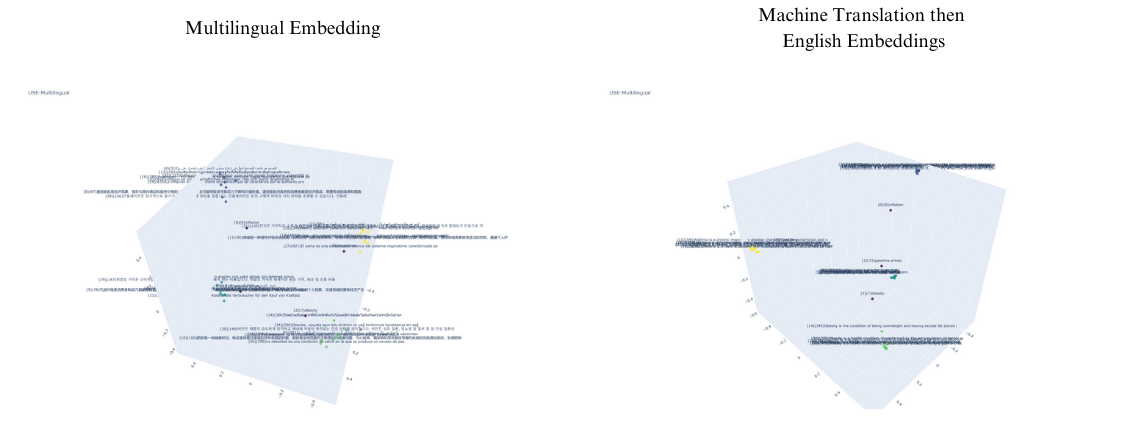
\includegraphics[width=1 \linewidth]{assets/comp_multi.png}
    \caption{comparison between Multilingual Embeddings and Machine Translation then English Embeddings over different dialects}
    \label{fig:comp_multilingual}
\end{figure}
\vskip 0.5cm
By translating all words to English and then using English language embeddings, the system makes sure that the language model can use its training effectively and give the best responses in the RAG pipeline.
%By translating all text into English and then applying English language embeddings, the system ensures that the language model can fully leverage its training and provide the most accurate and informative responses possible within the RAG pipeline.
\end{itemize}
\subsection{Table extraction}
In the RAG pipeline, extracting tables involves carefully finding and getting data from tables, as well as keeping the titles or captions that give information about the tables.
%Table extraction within the RAG pipeline is a meticulous process that involves not only the identification and retrieval of tabular data but also the preservation of its descriptive context, typically provided by accompanying titles or captions.
\vskip 0.5cm
\begin{itemize}
\item \textbf{Identifying and Extracting Tables with Titles}: The first step is to scan the Word document for tables, which are important for analyzing PPP projects. Beside every table, the system also takes out the title or caption that goes with it, often found right above the table in the document. The title is important because it gives a summary or focus of the content in the table, serving as a key to understanding the data. By taking out the table and its title together, the system keeps all the information intact. This helps users to know the meaning and importance of the data.The process begins by scanning the Word document for tables, which are often pivotal in conveying structured, quantitative data essential for PPP project analysis. Alongside each table, the system also extracts the associated title or caption, which is frequently located directly above the table in the document. This title is key to understanding the table's content as it often provides a summary or highlights the focus of the tabular data. By extracting the table and its title in tandem, the system retains the full context, allowing users to understand the purpose and implications of the data within.
\vskip 0.5cm
\item \textbf{Transformation into HTML Format}: After a table and its title are extricated, they experience a change into an HTML (Hypertext Markup Language) format . HTML is chosen since of its various leveled structure, which adjusts well with the inalienable structure of tables. It permits for the representation of complex information in a settled , discernable arrange that's both human readable and machine parseable.
\vskip 0.5cm
This change is guided by standards laid out in research on the representation of tabular data for large language models. For example, the approach recommended within the research paper "Table Meets LLM: Can Large Language Models Understand Structured Table Data? A Benchmark and Empirical Study" \cite{w14} serves as a guide for this process. The paper explains ways to show tables better so that the language model can understand and work with them more easily, \textbf{The Figure \ref{fig:html}} from this paper presents the final findings of different types of transformations and their result across different llm table understanding benchmarks.
%This transformation is guided by principles laid out in research on the representation of tabular data for large language models. For instance, the approach recommended in the research paper "Table Meets LLM: Can Large Language Models Understand Structured Table Data? A Benchmark and Empirical Study" \cite{w14} serves as a reference for this process. The paper details methods for effectively representing tables in a manner that improves the language model's comprehension and interaction with tabular structures.
\begin{figure}[H]
    \centering
    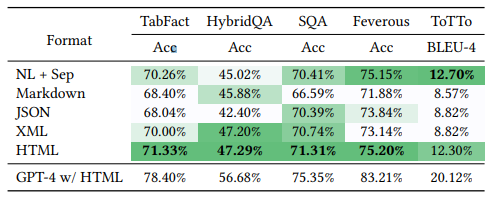
\includegraphics[width=0.9 \linewidth]{assets/html_res.png}
    \caption{Results of different transformations on LLM table understanding benchmarks}
    \label{fig:html}
\end{figure}

\vskip 0.5cm
When we transform tables to HTML format, each part of the table (cell, row, and column) is put inside special HTML tags. This makes a tree like structure that shows the table's layout accurately. The HTML format clearly separates data points, which helps the language model access and understand the table s contents accurately.
%In converting tables to XML, each cell, row, and column is encapsulated within XML tags, creating a tree-like structure that accurately reflects the table's layout. The XML format provides clear demarcations of data points, which is crucial for the language model to navigate and understand the table's contents accurately.
\vskip 0.5cm
\item \textbf{Preparation for LLM Interpretation}: The table is represented in HTML format to help the language model work with tabular data more effectively. This helps the LLM to better use the data from the table during conversations. It gets really good at using and making connections between the tabular data and the text or questions it comes across.%The XML representation of the table ensures that when the language model encounters tabular data, it has a structured and semantically rich format to work with. This enables the LLM to process and integrate the data from the table more effectively into the conversational context. It becomes adept at referencing specific entries and drawing connections between the tabular data and the textual or conversational queries it encounters.
\end{itemize}
\vskip 0.5cm
The RAG pipeline improves the chatbot's ability to use structured data by changing tables and titles into a format that works well with language models. This step makes sure that the chatbot can understand numbers and patterns as well as written words. This helps the chatbot give better and more detailed responses when analyzing PPP projects.
% %By extracting tables along with their titles and converting them into a language model-friendly XML format, the RAG pipeline enhances the chatbot's capability to process and utilize structured data. This step ensures that numerical and structured insights are as accessible and understandable to the chatbot as textual information, leading to more informed and comprehensive responses in the analysis of PPP projects.
% %-----------------------------------------------------

\section{Data Embedding}
Word embeddings are key concept in NLP, a fieldin machine learning. Word embeddings convert text data into numbers that machine learning algorithms can understand. can also help us understand the meaning of words in relation to other words. For example, \textbf{Figure \ref{fig:embed}} shows a example of embeddings in three dimensions. %\cite{w15}.
%Word embeddings are a key concept in natural language processing (NLP), a field within machine learning. Word embeddings transform textual data, which machine learning algorithms can’t understand, into a numerical form they can comprehend. In addition, they can be used to capture the contextual essence of words, their semantic and syntactic similarity, and their relation with other words. For instance, Figure 4.2 illustrates a sample of embeddings in three dimensions\cite{w15}.
\vskip 0.5cm
Before embedding, the document must be divided into smaller sections or chunks, so it can be analyzed and processed more easily. Chunking is play a pivotal role in helping with remembering and creating things quickly. These pieces are then dealt with separately, making it easier to find and create specific information.
%Befor embedding, the document must be broken down into smaller, more manageable segments or "chunks," facilitating focused analysis and processing of the text. the chunking plays a pivotal role in managing the retrieval and generation processes efficiently. These chunks are then processed individually, allowing for more focused retrieval and generation.

\begin{figure}[H]
    \centering
    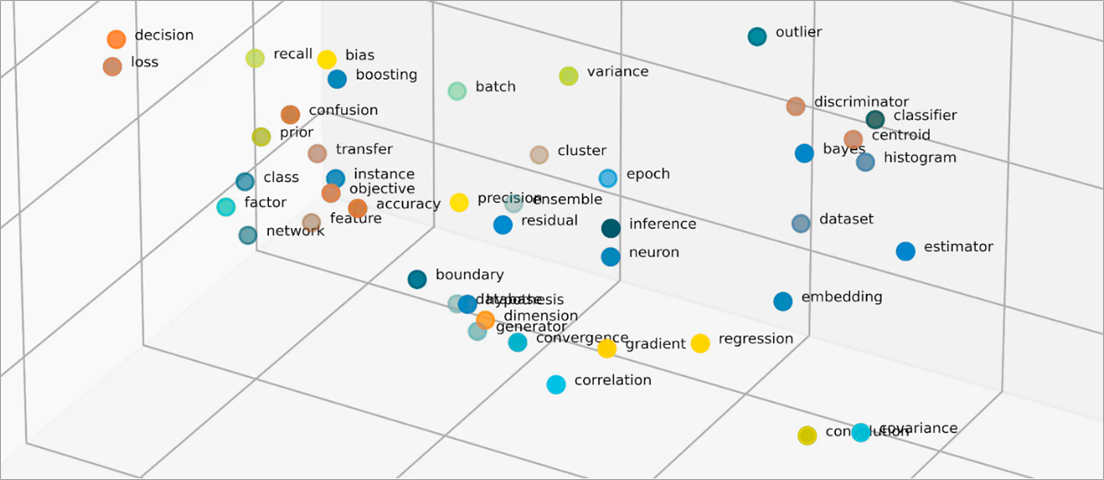
\includegraphics[width=1 \linewidth]{assets/3-d embed.png}
    \caption{Three-dimension embedding sample}
    \label{fig:embed}
\end{figure}
\subsection{Choice of embedding model}
Choosing the right embedding model is very important, especially when working with English documents. The model must be good at understanding the language and specialized terms used in legal and financial documents.
%The choice of the appropriate embedding model is crucial, especially when dealing with documents in the English language. The model must not only accurately capture the nuances of the language but also be adept at interpreting the specialized terminology used in legal and financial documents.
\vskip 0.5cm
The BGE M3 model, mentioned in the article "OpenAI vs. Open Source Multilingual Embedding Models "\cite{w16}, makes a strong argument for why it should be chosen. This model is very good at understanding many different meanings in English because it has been trained on lots of different types of data from lots of different areas. \textbf{The figure \ref{fig:embed_comp}} shows the comparison between different models and their performance on Mean Reciprocal Rank (MRR) which is an evaluation benchmark for embedding models.
\begin{figure}[H]
    \centering
    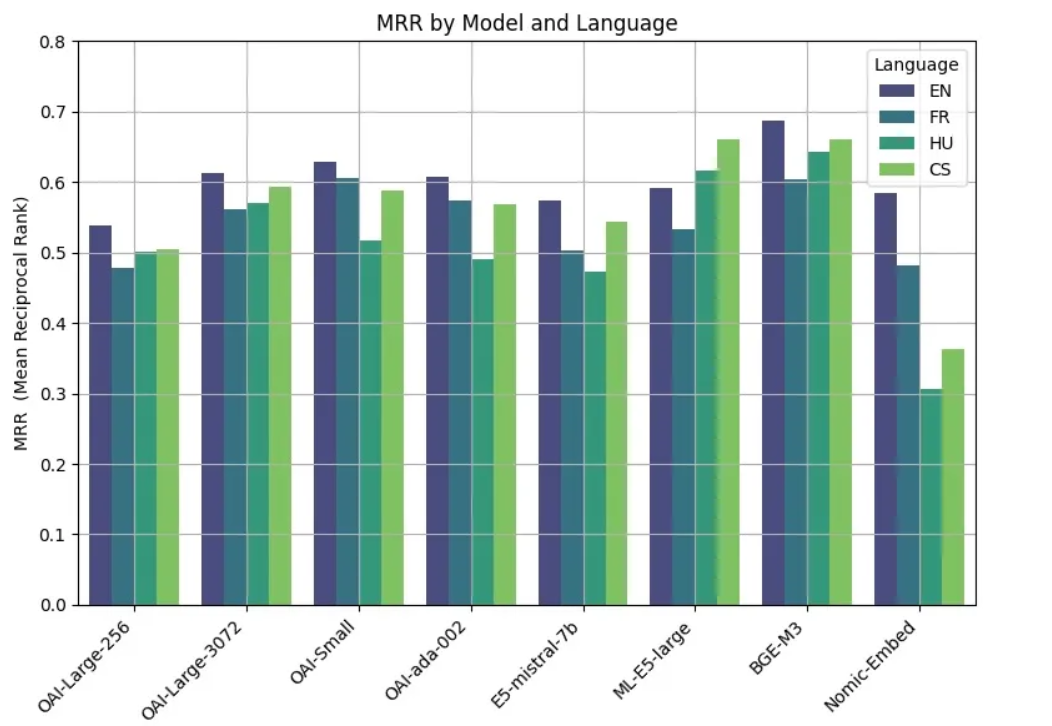
\includegraphics[width=1 \linewidth]{assets/embed_md_comp.png}
    \caption{performance of the latest embedding models on Mean Reciprocal Rank (MRR) benchmark}
    \label{fig:embed_comp}
\end{figure}
%The BGE-M3 model, discussed in the article "OpenAI vs. Open Source Multilingual Embedding Models" \cite{w16}, presents a strong case for its selection. This model is notable for its ability to encapsulate a wide spectrum of nuances in English, given its training on diverse datasets encompassing various domains and contexts.
\vskip 0.5cm
\textbf{Choosing BGE-M3 for English Language Embeddings:} The BGE-M3 model is special because it is part of a group of models that are made to really understand language well, , stands out for several reasons:%The BGE-M3 model, part of the larger family of models that are designed to be both broad and deep in their understanding of language, stands out for several reasons:
\vskip 0.5cm
\begin{enumerate}
    \item \textbf{Model Specifications:} The BGE-M3 model, identified as BAAI/bge-m3, has a dimension of 1024 and can process sequences up to 8192 tokens in length. It is a multilingual model that benefits from a unified fine-tuning approach, incorporating techniques such as dense, sparse, and colbert tuning. These features are derived from its unsupervised learning capabilities, enhancing its versatility and adaptability across various text analyses.
\vskip 0.5cm
\item \textbf{Contextual Understanding:} It has been trained to understand context well, which is important for reading PPP documents that often contains complicated language structures.%It has been trained to comprehend context deeply, which is essential for parsing PPP documents that often contain dense and intricate language structures.
\vskip 0.5cm
\item \textbf{Semantic and Syntactic Awareness:} The BGE-M3 model captures how words are related, which is important when dealing with technical language where accuracy is very important.%The BGE-M3 model captures the semantic relationships between terms, a crucial feature when dealing with technical language where precision is paramount.
\vskip 0.5cm
\item \textbf{Robust Training:} The training process for BGE-M3 has helped the model learn different language patterns, so it can handle new words and ways of speaking easily.%The training regime for BGE-M3 has exposed it to a variety of linguistic patterns, making it robust when dealing with unexpected ways of expression or new terminology.
\vskip 0.5cm
\item \textbf{Efficiency in Processing:} As PPP documents can be very long and complicated, the ability of BGE M3 to process a lot of text quickly is a big benefit, making sure the system stays fast.%As PPP documents can be lengthy and complex, the efficiency of BGE-M3 in handling large volumes of text is a significant advantage, ensuring that the system remains responsive.
\end{enumerate}
\vskip 0.5cm
In summary, the strategic selection of BGE-M3 for English language embeddings helps us analyze PPP project documents better. It makes sure we can use a platform that gives us lots of specific information, context, and accurate insights necessary for informed decision-making.
%In summary, the strategic selection of BGE-M3 for English language embeddings, helps us in providing a nuanced and efficient tool for analyzing PPP project documents. It ensures that we have access to a platform capable of delivering detailed, contextually rich, and accurate insights necessary for informed decision-making.
\subsection{Chunking and embedding for different type of data}
Before embedding, documents are chunked (divided) into smaller segments. This step before the main process is important for controlling the system's workload and helps to find information in a detailed way. Breaking down the text into smaller parts helps the system find and organize information better, making it easier to search for specific content. This approach helps prevent losing important information when dealing with long texts. Each piece of information is carefully looked at.
%Before embedding, documents are chunked into smaller segments. This pre-processing step is instrumental in managing the system's load and allows for a granular approach to information retrieval. By breaking down the text into manageable chunks, each segment can be embedded and indexed individually, which enhances the system's ability to retrieve and generate precise and relevant content. This approach also mitigates the risks of information loss that can occur when handling large blocks of text, ensuring that each piece of information is given due consideration.
\vskip 0.5cm
In our RAG pipeline, Multi Representation Indexing is a very important step where we map different types of data, like text and tables, to their own vector representations. This process makes it easy to find information and ensures you can remember everything.
%In our RAG pipeline, Multi-Representation Indexing is the crucial step where different data types—namely text and tables—are mapped to their respective vector representations. This process allows for a seamless retrieval experience that ensures comprehensive data recall.
\subsection{Tables Chunking and Embedding}
The  multi-representation indexing approach  in our system is designed to handle the complicated table data in PPP documents. Here, the term multi-representation shows that the pipeline can store different types of data, such as vector summaries of tables and the tables themselves.
%The multi-representation indexing approach in our pipeline is designed to effectively handle the complex nature of table data embedded from PPP documents. Here, the term "multi-representation" reflects the pipeline's capacity to index various forms of data, particularly the vector representations of table summaries and the actual tables themselves.
\vskip 0.5cm
\begin{itemize}
    \item \textbf{Process of Indexing Table Embeddings:} When we put the tables into the system, we create vector summaries of the important information in the tables. These summaries are stored in a database called PgVector which can handle vector data. This process involves making a map between a high-dimensional vector space and the original table. Each vector is a point in this space, representing the meaning and information in a table summary. By indexing these vectors, we make it easier to find things quickly when looking for specific information through semantic queries.%Upon embedding the tables, the resulting vector representations — summaries that capture the essential information within the tables — are indexed in a database designed to handle vector data, such as PgVector. This indexing process involves creating a map between the high-dimensional vector space and the original tabular data. Each vector is a point in this space, representing a table summary's semantic and informational content. By indexing these vectors, we facilitate a highly efficient retrieval process, where searching for information through semantic queries becomes possible.
    \item here we choose the llmm (comp table)
    \item \textbf{Retrieval of Full Table Data:} The strength of multi-representation indexing is that it able to link these vectors back to all the data in the table. When a user needs specific information, the system can find the right data and get the complete table. This means that users will get a short answer to their questions and also be able to look at all the detailed information in the table to get a better understanding.%The strength of multi-representation indexing lies in its ability to associate these vectors back to the full table data. When a user's query necessitates specific data retrieval, the system can quickly locate the relevant vector in the indexed space and then pull the complete table from the repository. This ensures that users not only receive a summary response to their queries but can also access the detailed data within the table for comprehensive insights.
\end{itemize}

\subsection{Text Chunking and Embedding}
The sophisticated architecture of our RAG pipeline can handle different types of text data from PPP documents using a method called multi-representation indexing. This means the pipeline can organize various kinds of data, especially focusing on the vector representations of small text pieces and the longer text segments they come from(parent chunck).
%The sophisticated architecture of our RAG pipeline accommodates the varied and layered texture of textual data extracted from PPP documents through a method known as "multi-representation indexing." This term encapsulates the pipeline's ability to meticulously index different forms of data, specifically focusing on the vector representations of small textual chunks and the full-bodied text segments from which they are derived.
\vskip 0.5cm
\begin{itemize}
    \item \textbf{Chunking for Text Embedding:} For this process, we are using Recursive text splitting which involves breaking down a big piece of text into smaller chunks. This is really helpful when working with long documents, because it helps the system to manage and process data while still keeping important information in context.%For this processes we are usign Recursive text splitting which is an iterative process where a larger body of text is progressively broken down into smaller segments or chunks. This is particularly useful when dealing with extensive documents, as it allows the system to manage and process data in a way that balances context retention with manageable analysis sizes.
    \vskip 0.5cm
    The process starts by breaking the document into big chunks, each containing up to 3000 tokens. This initial size of each chunk is set in order to make sure that each part has enough information to accurately show the details of the text.
    %The process begins with the initial splitting of the document into large chunks, each up to 3000 tokens in size. This initial chunk size is chosen to ensure that each segment maintains enough contextual information, which is essential for the embeddings to accurately represent the nuances of the text.
    \vskip 0.5cm
    After this first pass, these large chunks may still be too broad for the fine-grained analysis and retrieval purposes of our system. Therefore, the large chunks undergo a second round of recursive text splitting, where they are further divided into smaller chunks, each consisting of approximately 200 tokens. This size is optimized for the embedding process, where each small chunk is then transformed into a vector representation that captures the semantic richness of the text within that segment.
    \item \textbf{Multi-Representation Indexing:} In our pipeline, both levels of chunked data—large (3000-token) chunks and small (200-token) chunks—are important. The small chunks are embedded and the vectors produced from these embeddings are indexed. However, when it comes to retrieval, the system uses multi-representation indexing to ensure that it can return information from the larger chunks.
    \vskip 0.5cm
    The selection of recursive text splitting and multi representation indexing offers a highly productive approach to handling broad PPP documents. By breaking content into both large and small chunks and embedding these for point by point indexing , the framework adeptly balances comprehensive information analysis with the require for holding relevant information. This technique guarantees that the retrieval process is robust and exact.
\end{itemize}
%definition for the vectorstore its utility and how it helps us for the development of our ai assistance
%how we chose our db 
%what is the differnce between relationnal db and vectorstore.
%etc




\section{History-Aware Conversation with Document}
Within the domain of interactive AI frameworks , the capacity to review and construct upon past saved interactions is fundamental for keeping up a coherent and significant discourse . Typically where History Aware Conversation Management comes into play inside our Rag pipeline, especially within the context of engaging with PPP reports.
\vskip 0.5cm
\begin{enumerate}
    \item \textbf{Selective Document Interaction:} Inside our Rag pipeline, the selection of a particular document to interact with is essential. It engages users to lock in specifically with a specific PPP feasibility report from an established store associated to Jade's OneDrive collection and also save their chat history to our database. The user can choose and search for a report, then they can start a unique conversational thread with that document. This interaction isn't generic but profoundly personalized, permitting the user to inquiry and speak with the content of the chosen report as in case it were a knowledgeable partner. 
    \vskip 0.5cm
    \item \textbf{Question Translation and Reformulation for Context Awareness:} After selecting the document, then the users can pose questions in various languages, the system adeptly translates these into English, using advanced models to ensure nuanced accuracy. This translation is then fused with the document's chat history, providing the large language model (LLM) with a rich contextual backdrop. The LLM may reformulate the inquiry for enhanced context specificity, drawing from previous dialogues and document details to craft questions that elicit more precise information. This consistent use of English across the board maintains the system's processing uniformity, ensuring each user receives context-aware, insightful responses from the conversational AI.
\end{enumerate}

\section{Integrated Retrieval and Re-Ranking}
Within the Rag pipeline, the integrated retrieval and re ranking process plays a essential part in improving the system s response quality. This stage takes after the extraction and embedding stages where both tables and content chunks are indexed and made searchable.
\subsection{Similarity Search on Indexed Documents}
The Similarity Search stage could be a pivotal component of the Rag pipeline, where the system s capacity to accurately and productively coordinate user questions to the most significant information comes into play.
\vskip 0.5cm
\begin{enumerate}
    \item \textbf{Mechanism of Similarity Search:} Upon accepting a query , the system takes the user s input into a query vector utilizing the same embedding model applied to the text and table information during the indexing stage . This vector represents the semantic signature of the query.
    \vskip 0.5cm
    \item \textbf{Finding the Best Match:} The multi representation indexed archives make a searchable space, our vector store (PgVector). Comprising of vectors for each chunk of content and table information. Each vector acts as a arrange in this high dimensional space, encoding the semantic essence of the corresponding text or table.
    \vskip 0.5cm
    The system conducts a search inside this vector space to distinguish the vectors that are closest to the query vector those with the highest degree of semantic similarity . This similitude is regularly computed utilizing metrics such as cosine similarity , which measures the cosine of the angle between two vectors, showing how closely aligned the implications of the query and the archive chunks are. For example, \textbf{Figure \ref{fig:vec_search}} shows a vector representation of kitten query and how it's close to other animals representation especially to cat and dog.
    \vskip 0.5cm
    \begin{figure}[H]
        \centering
        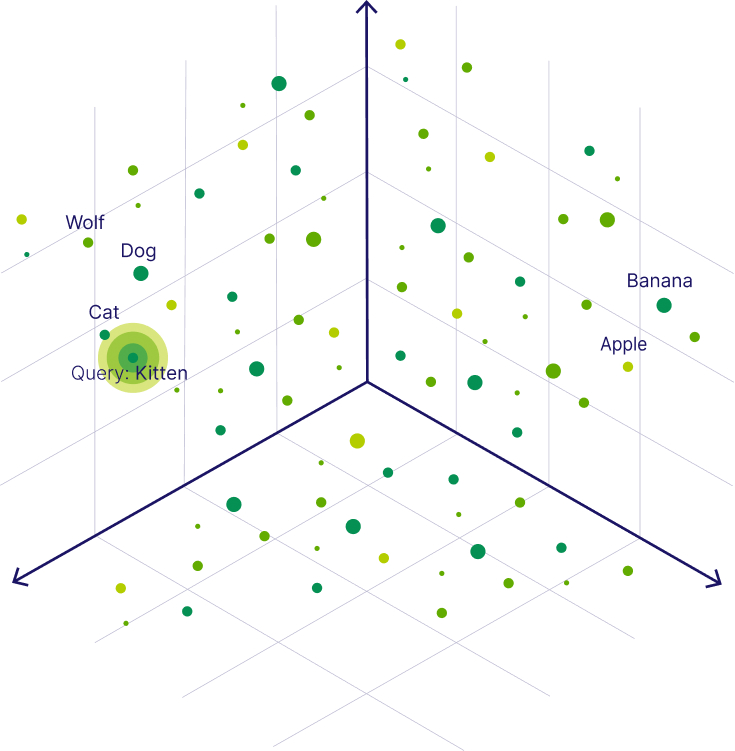
\includegraphics[width=0.8 \linewidth]{assets/vec_search.jpg}
        \caption{Vector representation of kitten query and how it's close to other animals representation in a 3 dimensional space}
        \label{fig:vec_search}
    \end{figure}
    \vskip 0.5cm
    The closest vectors are at that point mapped back to their original content chunks or table information . This retrieval is the primary step in giving a response to the user s query , sourcing the foremost semantically aligned pieces of data from the complete corpus of indexed documents .
\end{enumerate}
The Similarity Search on Indexed Reports may be a confirmation to the power of vector space modeling in understanding and retrieving data. It empowers the system to filter through endless amounts of information with precision and return the foremost pertinent data, hence streamlining the user's experience in exploring complex PPP reports.
\subsection{RAG Fusion for Contextual Alignment}
RAG Fusion is an advanced technique in the RAG pipeline that harnesses the strengths of ensemble methods and reciprocal rank fusion for superior data retrieval.
\vskip 0.5cm
At it's core RAG Fusion uses Reciprocal Rank Fusion (RRF) which is an integral component within the context of Rag fusion that essentially contributes to the efficiency and accuracy of the retrieval process within the pipeline. Its execution inside the Rag system offers a method for combining the strengths of distinctive retrieval models to ensure the foremost important data is surfaced in response to a user's inquiry.
\begin{itemize}
    \item \textbf{Fundamentals of Reciprocal Rank Fusion (RRF):} RRF is based on the principle that the significance of a document can be inversely relative to its positioning over diverse retrieval models. The method was detailed in a research paper by Cormack, Clarke, and Buettcher,titled "Reciprocal Rank Fusion Outperforms Condorcet and Individual Rank Learning Methods"\cite{w17}. It s an successful data fusion strategy that totals different positioned lists into a single, more exact ranking.
    \vskip 0.5cm
    \item \textbf{How RRF Works:} In RRF, each document's rank from the individual result sets is converted into a score using the reciprocal of its rank. This means that if a document is ranked first in any retrieval model's list, it's assigned a score of 1; if it's ranked second, it gets a score of 1/2, and so on. These scores are then summed across all retrieval models for each document. The documents are then re-ranked based on these composite scores, with higher scores indicating higher relevance. This is the RRF equation
    \vskip 0.5cm
    \[
\text{RRFscore}(d \in D) = \sum \left[ \frac{1}{k + r(d)} \right]
\]

\text{where:}
\begin{itemize}
  \item \( d \) represents a document within the set \( D \) of documents.
  \item \( k \) is a constant that helps to balance between high and low ranking documents.
  \item \( r(d) \) is the rank or position of the document \( d \).
\end{itemize}
\item \textbf{Contribution to our RAG Pipeline:} The application of RRF in the RAG pipeline enhances the retrieval process by allowing the system to effectively combine and leverage the insights from our two different retrievals, the text retrieval and table retrieval . This is particularly useful in the RAG framework, where diverse data formats and complex query contexts can lead to varying retrieval performances across different models and with RRF we can have a unified set of score for each chunk returned whether it is a text chunk or a table.
\end{itemize}
\vskip 0.5cm
The RRF method enhances the RAG fusion process by adeptly amalgamating the strengths of varied retrievals, ensuring the system’s effectiveness over diverse datasets. Its application is pivotal in re-ranking the information chunks retrieved, which is essential for furnishing the most contextually relevant and reliable answers to complex inquiries. By reordering these data chunks, RRF helps to align the output more closely with the user's original intent.
\vskip 0.5cm
The effectiveness of RRF in reordering content for LLMs can be further understood through the lens of the research paper "Lost in the Middle: How Language Models Use Long Contexts"\cite{w18}. This study underscores the challenges and solutions in how LLMs handle extended contexts. LLMs are often designed to prioritize information at the top and the end of a user query as being more relevant, which might not always align with the user's needs. We can mitigate this by re-ranking the data chunks, placing those with the highest relevance at the start and end of our query. This tailored reordering can lead to more coherent and contextually rich responses from the LLM. \textbf{Figure \ref{fig:lost_in}} from this study shows how Changing the location of relevant information within the language model’s input context gives different results.
\begin{figure}[H]
    \centering
    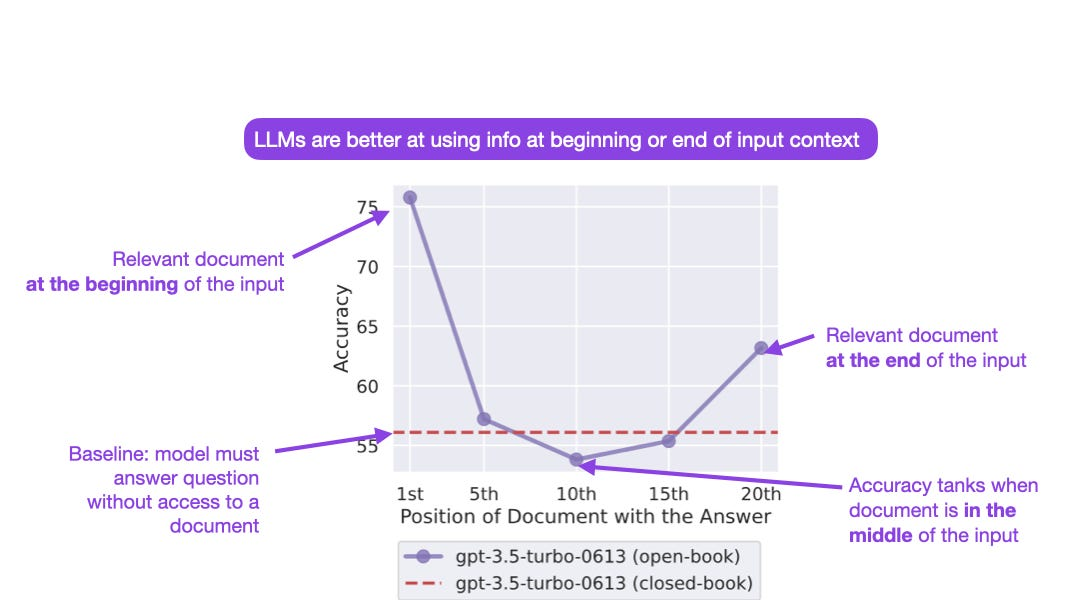
\includegraphics[width=1 \linewidth]{assets/lost_in.jpg}
    \caption{Result of changing the position of the passage that answers an input question}
    \label{fig:lost_in}
\end{figure}
\vskip 0.5cm
In essence, RRF acts as a strategic intermediary in the RAG fusion process, optimizing the arrangement of data chunks fed into the LLM. This optimization facilitates the generation of better-informed answers, effectively harnessing the long-context capabilities of LLMs to provide users with precise and contextually nuanced responses.
\section{Answer Generation}
\section{RAG system Evaluation}
%Explanation of evaluation metrics and methodologies for assessing the performance of RAG systems.
%Presentation of experimental results and analysis of system performance.

\section{conclusion}





